\documentclass{standalone}
%<--------------------------------------------------------------------------->%
%%% Color %%%
\usepackage[dvipsnames]{xcolor} % \textcolor{red}{}
\definecolor{rot}{RGB}{229,0,0}
\definecolor{bla}{RGB}{0,98,144}
\definecolor{gel}{RGB}{255,195,0}
%<--------------------------------------------------------------------------->%

%<--------------------------------------------------------------------------->%
%%% TikZ %%%
\usepackage{tikz}
\usetikzlibrary{calc}
\usetikzlibrary{angles,quotes}
% \usetikzlibrary{intersections,topaths}
% \usetikzlibrary{decorations.markings}
%<--------------------------------------------------------------------------->%
%%% TikZ: Mark Angles %%%
\newcommand{\MarkRightAngle}[5][]{%
\draw[#1] let \p1=($(#3)-(#4)$),\n1={1/veclen(\x1,\y1)},\p2=($(#4)-(#5)$),\n2={1/veclen(\x2,\y2)} in%
($(#4)!#2!(#5)$) -- ++(\x1*\n1*#2,\y1*\n1*#2) -- ++(\x2*\n2*#2,\y2*\n2*#2);}
\newcommand{\MarkAngle}[5]["$\theta$",->,draw=blue!80,fill=blue!20]{\pic[#1,angle radius=#2] {angle = #3--#4--#5};}
%<--------------------------------------------------------------------------->%

\begin{document}

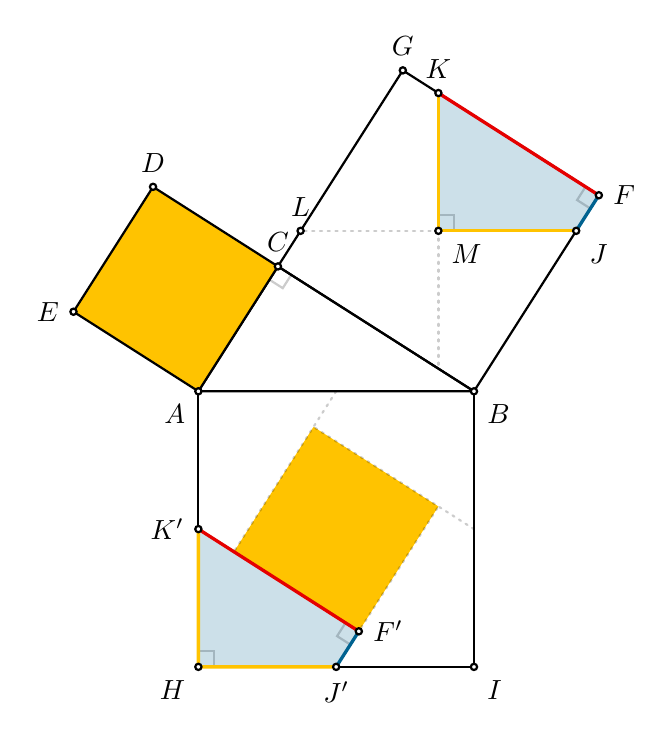
\begin{tikzpicture}[thick,line cap=round]
	\tikzstyle{jiao}=[solid,circle,draw,fill=white,inner sep=.8pt];
	\tikzstyle{rightangle}=[opacity=0.2];
\newcommand{\rightanglesize}{0.2cm}
\tikzstyle{normalangle}=[fill=bla,opacity=0.2];
\newcommand{\anglesize}{0.5cm}
\tikzstyle{help}=[dotted,opacity=0.2];
%<--------------------------------------------------------------------------->%

	\newcommand{\length}{3.5cm}
	\coordinate (A)  at (0,0);
	\coordinate (B)  at (\length,0);
	\coordinate (C)  at ($(\length/2,0)+(115:\length/2)$);
	\coordinate (D)  at ($(C)!1!-90:(A)$);
	\coordinate (E)  at ($(A)!1!90:(C)$);
	\coordinate (F)  at ($(B)!1!-90:(C)$);
	\coordinate (G)  at ($(C)!1!90:(B)$);
	\coordinate (H)  at ($(A)!1!-90:(B)$);
	\coordinate (I)  at ($(B)!1!90:(A)$);
	\coordinate (M)  at ($(B)!0.5!(G)$);
	\coordinate (BC) at ($(M)-(0,\length/2)$);
	\coordinate (FG) at ($(BC)!2!(M)$);
	\coordinate (CG) at ($(M)!1!90:(FG)$);
	\coordinate (BF) at ($(CG)!2!(M)$);
	\coordinate (AH) at ($(A)!0.5!(H)$);
	\coordinate (AB) at ($(A)!0.5!(B)$);
	\coordinate (HI) at ($(I)!0.5!(H)$);
	\coordinate (BI) at ($(B)!0.5!(I)$);
	\coordinate (d)  at ($($(C)-(BC)$)+(BI)$);
	\coordinate (e)  at ($($(B)-(BF)$)+(AB)$);
	\coordinate (a)  at ($($(F)-(FG)$)+(AH)$);
	\coordinate (c)  at ($($(G)-(CG)$)+(HI)$);
	%% triangle
	\draw (A) -- (B) -- (C) --cycle;
	\draw (B) -- (F) -- (G) -- (C) --cycle;
	\draw (A) -- (H) -- (I) -- (B) --cycle;
	\draw[fill=gel] (A) -- (C) -- (D) -- (E) --cycle;
	\path[fill=gel] (a) -- (c) -- (d) -- (e) --cycle;
	%% Angles
	\MarkRightAngle[rightangle]{\rightanglesize}ACB;
	\MarkRightAngle[rightangle]{\rightanglesize}{BF}M{FG};
	\MarkRightAngle[rightangle]{\rightanglesize}IHA;
	\MarkRightAngle[rightangle]{\rightanglesize}{FG}F{BF};
	\MarkRightAngle[rightangle]{\rightanglesize}{AH}a{HI};
	%% Mark lines
	\draw[help] (HI) -- (c);
	\draw[help] (BI) -- (d);
	\draw[help] (AB) -- (e);
	\draw[help] (AH) -- (a);
	\draw[help] (M)  -- (CG);
	\draw[help] (M)  -- (BC);
	\draw[fill=bla,opacity=0.2] (F) -- (FG) -- (M) -- (BF);
	\draw[very thick,rot] (F) -- (FG);
	\draw[very thick,bla] (F) -- (BF);
	\draw[very thick,gel] (FG) -- (M) -- (BF);
	\draw[fill=bla,opacity=0.2] (a) -- (AH) -- (H) -- (HI);
	\draw[very thick,rot] (AH) -- (a);
	\draw[very thick,bla] (HI) -- (a);
	\draw[very thick,gel] (AH) -- (H) -- (HI);
	%% Final
	\node[jiao,label=below left  :{$A$} ] at (A)  {};
	\node[jiao,label=below right :{$B$} ] at (B)  {};
	\node[jiao,label=above       :{$C$} ] at (C)  {};
	\node[jiao,label=above       :{$D$} ] at (D)  {};
	\node[jiao,label=left        :{$E$} ] at (E)  {};
	\node[jiao,label=right       :{$F$} ] at (F)  {};
	\node[jiao,label=above       :{$G$} ] at (G)  {};
	\node[jiao,label=below left  :{$H$} ] at (H)  {};
	\node[jiao,label=below right :{$I$} ] at (I)  {};
	\node[jiao,label=below right :{$M$} ] at (M)  {};
	\node[jiao,label=right       :{$F'$}] at (a)  {};
	\node[jiao,label=below right :{$J$} ] at (BF) {};
	\node[jiao,label=below       :{$J'$}] at (HI) {};
	\node[jiao,label=above       :{$K$} ] at (FG) {};
	\node[jiao,label=left        :{$K'$}] at (AH) {};
	\node[jiao,label=above       :{$L$} ] at (CG) {};
\end{tikzpicture}

\end{document}
